% Captions for disease-partition-state-equations.tex visualization panels

\begin{figure*}[!htbp]
\centering
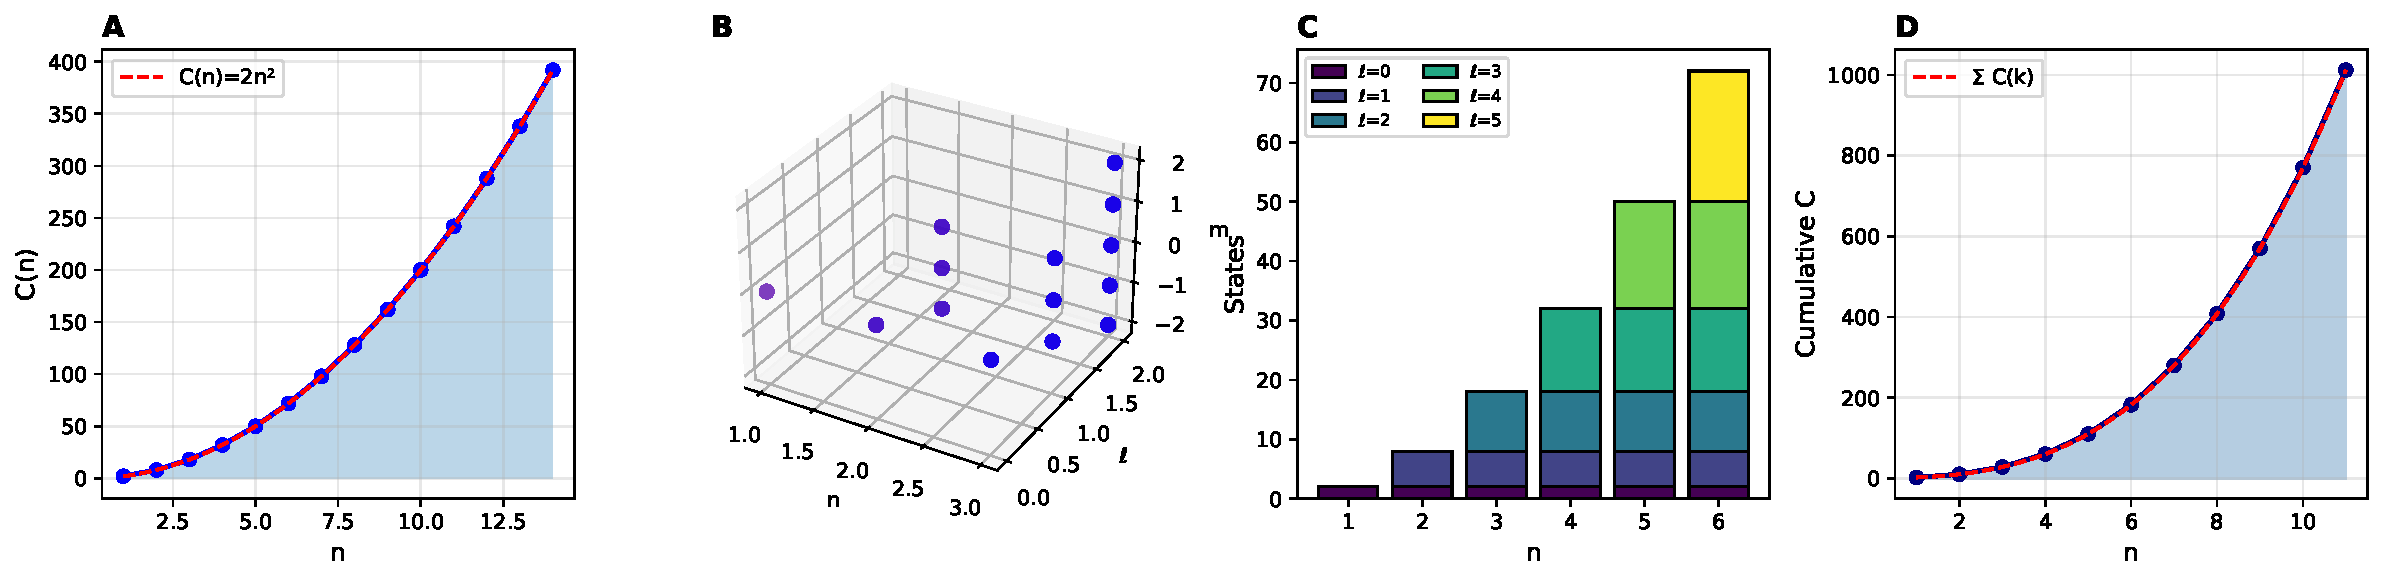
\includegraphics[width=0.9\textwidth]{figures/panel1_partition_structure.pdf}
\caption{\textbf{Partition Coordinate Structure and Capacity.}
\textbf{Panel A (left):} Partition capacity $C(n) = 2n^2$ as a function of depth coordinate $n$, showing quadratic growth from $C(1) = 2$ to $C(14) = 392$. The analytical form (red dashed) exactly matches computed values (blue circles), confirming the geometric derivation from spherical symmetry constraints.
\textbf{Panel B (center-left):} Three-dimensional visualization of partition state enumeration for $n \in \{1, 2, 3\}$, displaying all valid $(n, \ell, m)$ coordinate combinations. Blue and red points distinguish chirality $s = +\frac{1}{2}$ and $s = -\frac{1}{2}$ states respectively, illustrating the complete state space structure at each depth level.
\textbf{Panel C (center-right):} Stacked bar decomposition showing state count contributions by complexity coordinate $\ell$ at each depth $n$. Each $\ell$-subshell contributes $2(2\ell + 1)$ states, with the stack heights summing to $2n^2$, demonstrating the additive structure underlying partition capacity.
\textbf{Panel D (right):} Cumulative capacity $\sum_{k=1}^{n} C(k) = \frac{n(n+1)(2n+1)}{3}$ showing total accessible states up to depth $n$. This cubic scaling determines the information-theoretic capacity of the categorical observation framework.}
\label{fig:partition_structure}
\end{figure*}

\begin{figure*}[!htbp]
\centering
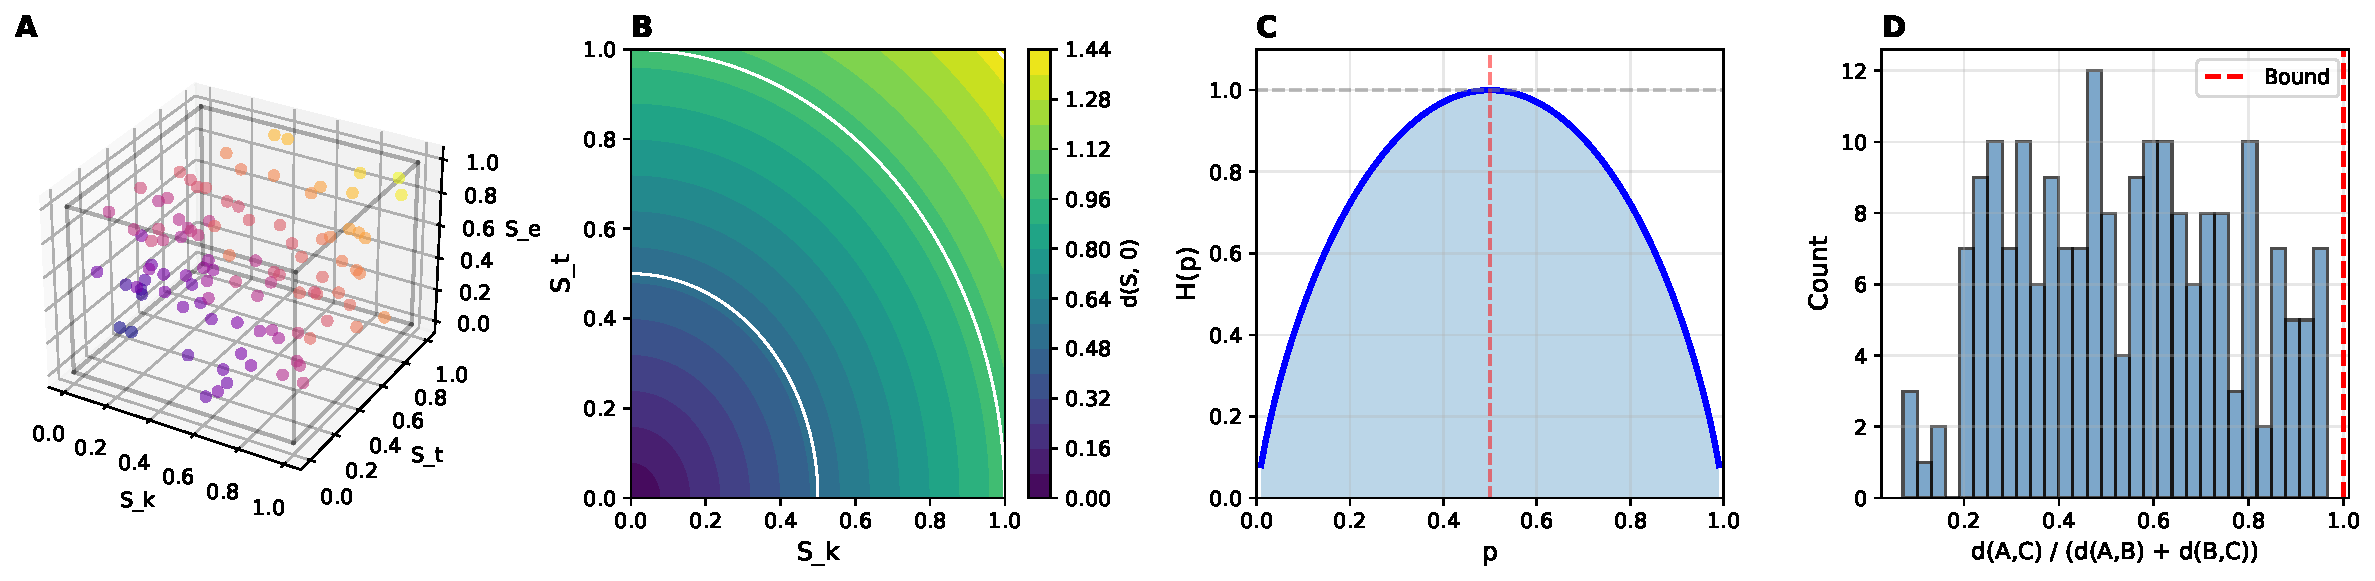
\includegraphics[width=0.9\textwidth]{figures/panel2_s_entropy.pdf}
\caption{\textbf{S-Entropy Space Geometry and Metric Properties.}
\textbf{Panel A (left):} Three-dimensional visualization of the S-entropy cube $\mathcal{S} = [0,1]^3$ with coordinates $(S_k, S_t, S_e)$ representing knowledge, temporal, and evolution entropy respectively. Randomly sampled states are colored by total entropy magnitude $\|S\| = \sqrt{S_k^2 + S_t^2 + S_e^2}$, illustrating the continuous state space available for trajectory evolution.
\textbf{Panel B (center-left):} Euclidean distance contours from the origin in the $(S_k, S_t)$ projection, with iso-distance curves at $d = 0.5, 1.0, 1.4$ shown in white. The flat metric structure enables straightforward distance computations for trajectory analysis and constraint verification.
\textbf{Panel C (center-right):} Binary Shannon entropy $H(p) = -p\log_2 p - (1-p)\log_2(1-p)$ as a function of probability $p$, demonstrating the information-theoretic foundation underlying S-entropy coordinates. Maximum entropy occurs at $p = 0.5$ (red dashed), corresponding to maximum uncertainty.
\textbf{Panel D (right):} Triangle inequality verification showing the distribution of ratio $d(A,C)/(d(A,B) + d(B,C))$ across 200 random point triplets. All ratios fall below 1.0 (red bound), confirming that S-entropy distance satisfies the metric axioms required for well-defined trajectory lengths.}
\label{fig:s_entropy}
\end{figure*}

\begin{figure*}[!htbp]
\centering
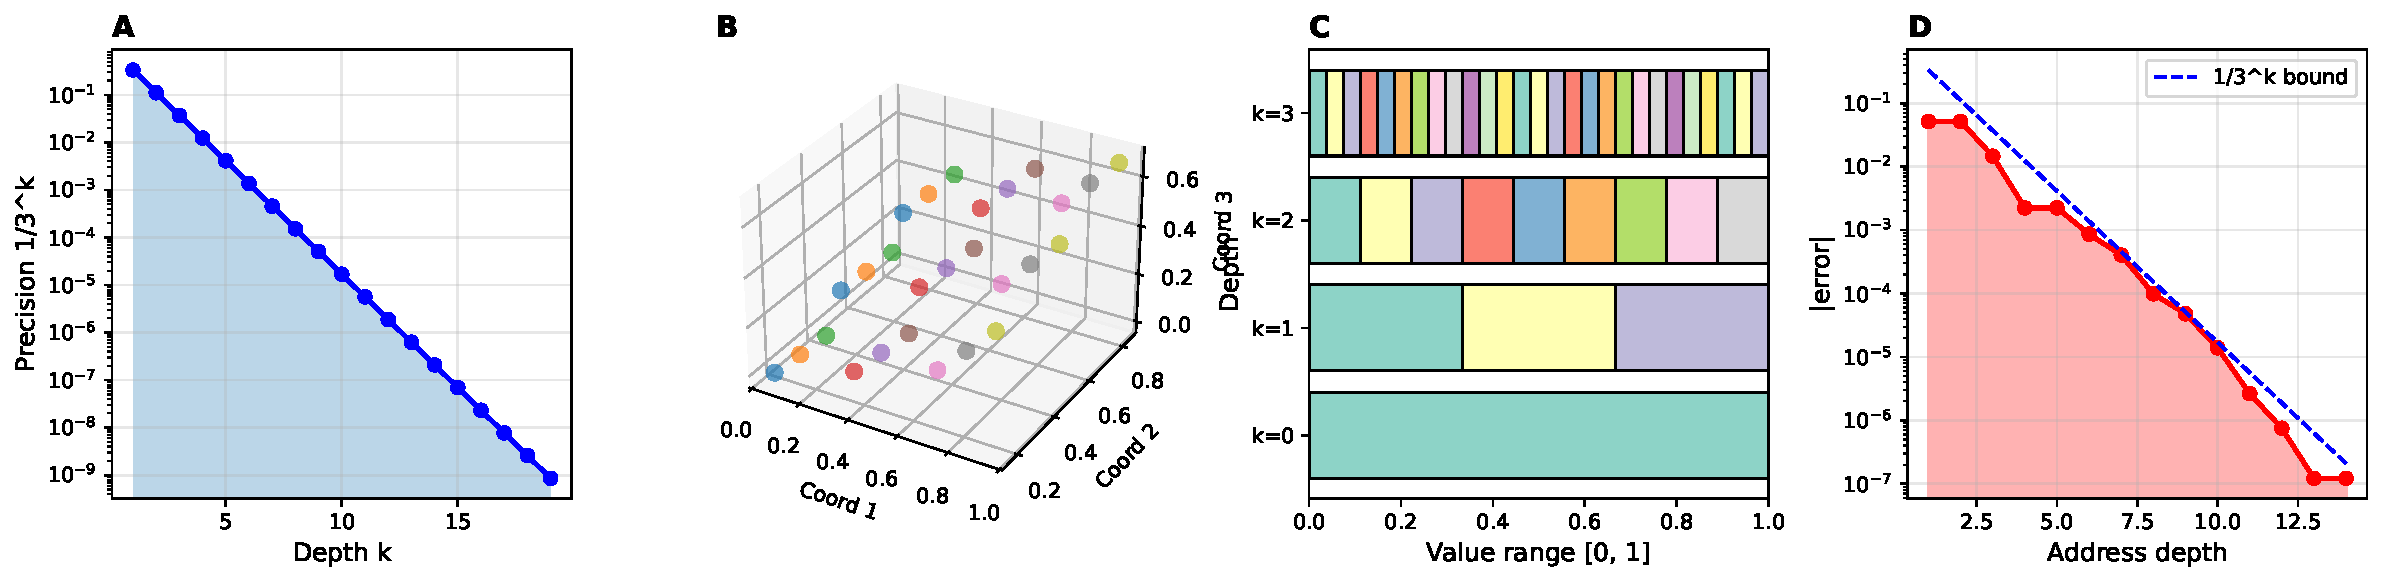
\includegraphics[width=0.9\textwidth]{figures/panel3_address_resolution.pdf}
\caption{\textbf{Ternary Address Resolution and Precision Scaling.}
\textbf{Panel A (left):} Address precision $\epsilon(k) = 3^{-k}$ on logarithmic scale as a function of depth $k$, demonstrating exponential refinement from $\epsilon(1) \approx 0.33$ to $\epsilon(19) \approx 10^{-9}$. This geometric progression enables arbitrary-precision value resolution through iterative categorical subdivision.
\textbf{Panel B (center-left):} Three-dimensional visualization of ternary address space partitioning at depth $k = 2$, showing how successive coordinate refinements subdivide the unit cube into $3^k = 9$ regions per dimension. Each point represents a resolvable address with distinct categorical coordinates.
\textbf{Panel C (center-right):} Hierarchical interval subdivision visualization showing ternary encoding at depths $k \in \{0, 1, 2, 3\}$. Each level subdivides intervals into three equal parts, creating the recursive structure underlying categorical address assignment.
\textbf{Panel D (right):} Resolution convergence demonstrating error $|v - \hat{v}|$ between target value $v = 0.718$ and resolved value $\hat{v}$ as a function of address depth. Observed errors (red) fall at or below the theoretical bound $3^{-k}$ (blue dashed), confirming the precision guarantees of the COMPLETE algorithm.}
\label{fig:address_resolution}
\end{figure*}

\begin{figure*}[!htbp]
\centering
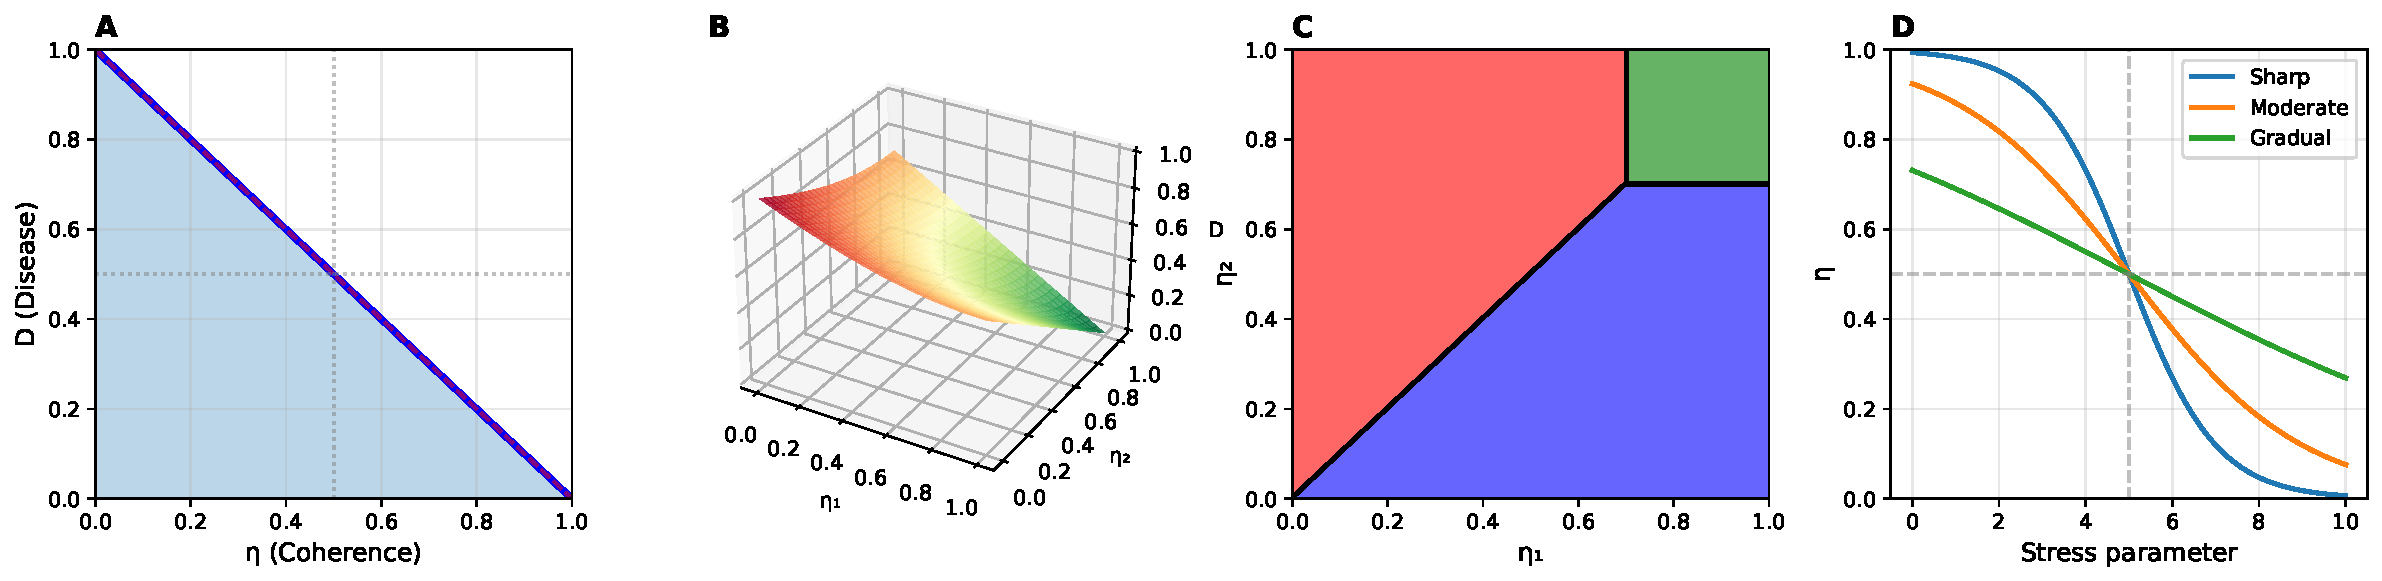
\includegraphics[width=0.9\textwidth]{figures/panel4_coherence_disease.pdf}
\caption{\textbf{Coherence-Disease Mapping and Classification Boundaries.}
\textbf{Panel A (left):} The fundamental transformation $D = 1 - \eta$ mapping coherence index $\eta \in [0,1]$ to disease index $D \in [0,1]$. This linear anti-correlation establishes that disease severity increases monotonically as coherence degrades, providing the quantitative foundation for disease state representation.
\textbf{Panel B (center-left):} Three-dimensional surface showing composite disease index $D = \sqrt{(1-\eta_1)^2 + (1-\eta_2)^2}/\sqrt{2}$ as a function of two coherence components. The surface geometry illustrates how multi-oscillator dysfunction combines to produce aggregate disease severity.
\textbf{Panel C (center-right):} Disease classification boundary regions in the $(\eta_1, \eta_2)$ coherence plane. Green indicates the healthy region where both $D_1, D_2 < 0.3$; red and blue regions indicate dominant disease types 1 and 2 respectively, with black curves marking classification boundaries where $D_1 = D_2$.
\textbf{Panel D (right):} Phase transition curves showing coherence response $\eta = 1/(1 + e^{(\sigma - 5)/k})$ to stress parameter $\sigma$ for different transition sharpness values $k$. Sharp transitions ($k = 1$) model acute dysfunction, while gradual transitions ($k = 5$) represent progressive disease onset.}
\label{fig:coherence_disease}
\end{figure*}

\begin{figure*}[!htbp]
\centering
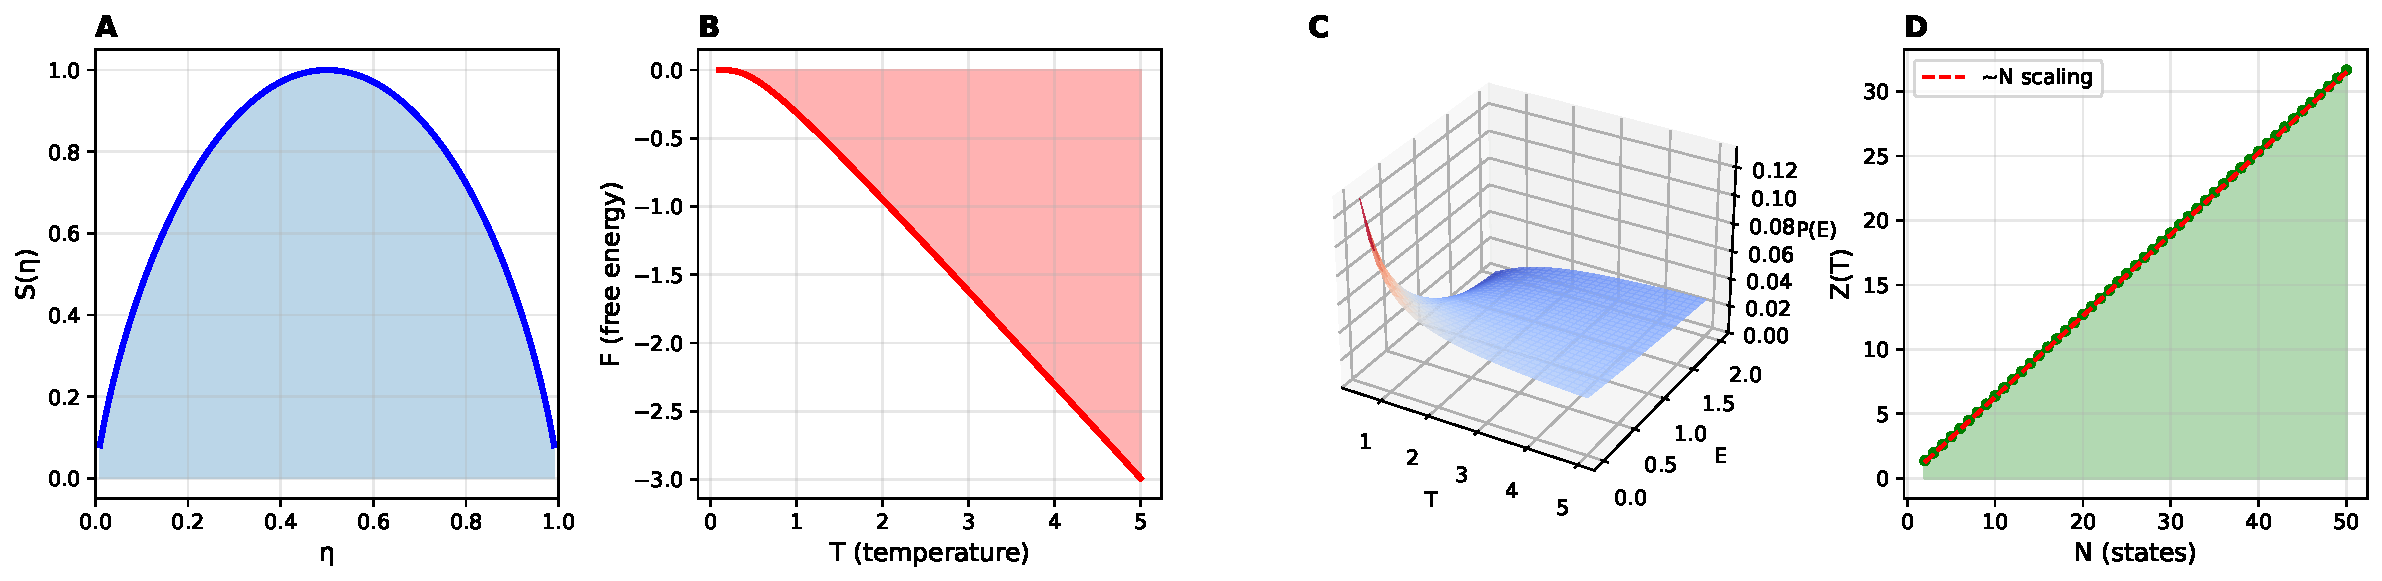
\includegraphics[width=0.9\textwidth]{figures/panel5_thermodynamic.pdf}
\caption{\textbf{Thermodynamic Connections and Statistical Mechanics Analogs.}
\textbf{Panel A (left):} Entropy-coherence relationship $S(\eta) = -\eta\ln\eta - (1-\eta)\ln(1-\eta)$ normalized to unit maximum, showing that intermediate coherence states ($\eta \approx 0.5$) correspond to maximum entropy while extreme states ($\eta \to 0$ or $\eta \to 1$) minimize entropy. This connects coherence dynamics to thermodynamic principles.
\textbf{Panel B (center-left):} Free energy analog $F = -T\ln Z$ for a two-state partition function $Z = e^{-E_0/T} + e^{-E_1/T}$ as a function of temperature $T$. The decreasing free energy with temperature parallels entropic stabilization in biological oscillator ensembles.
\textbf{Panel C (center-right):} Three-dimensional Boltzmann distribution surface $P(E) \propto e^{-E/T}$ showing occupation probability as a function of energy $E$ and temperature $T$. Higher temperatures flatten the distribution, analogous to coherence degradation under cellular stress.
\textbf{Panel D (right):} Partition function $Z(T)$ scaling with number of accessible states $N$ at fixed temperature $T = 1$. Linear scaling (red dashed) emerges from uniform energy spacing, connecting partition capacity to thermodynamic state counting.}
\label{fig:thermodynamic}
\end{figure*}

\begin{figure*}[!htbp]
\centering
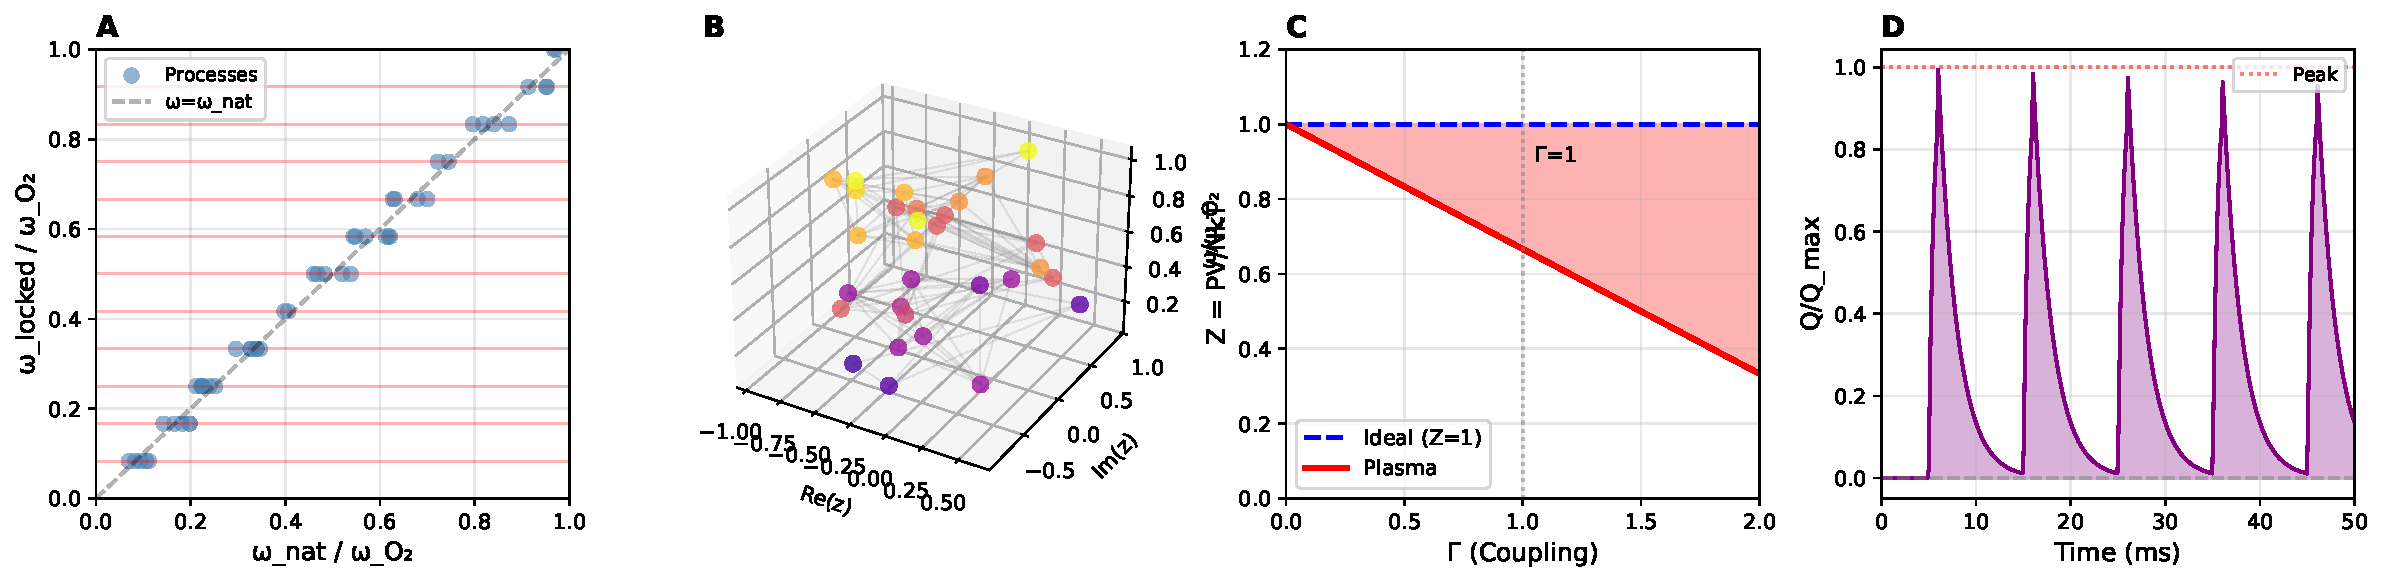
\includegraphics[width=0.9\textwidth]{figures/panel6_oxygen_charge.pdf}
\caption{\textbf{Oxygen Master Clock and Circuit Charge Dynamics.}
\textbf{Panel A (left):} Phase-locking of cellular processes to oxygen master clock harmonics $\omega_n = (n/N)\omega_{O_2}$. Natural frequencies $\omega_{\mathrm{nat}}$ (x-axis) map to discrete locked frequencies (y-axis) corresponding to the nearest harmonic (red horizontal lines). This frequency quantization creates the hierarchical clock structure with molecular oxygen as the master oscillator.
\textbf{Panel B (center-left):} Three-dimensional visualization of the phase-locked oscillator network, with each oscillator positioned by phase (x, y coordinates) and locked frequency (z-axis). Colors indicate frequency channel assignment, and connections link oscillators sharing the same harmonic, revealing the synchronization topology.
\textbf{Panel C (center-right):} Plasma coupling effects showing compressibility factor $Z = PV/Nk_BT$ as a function of Coulomb coupling parameter $\Gamma$. The ideal gas limit ($Z = 1$) is reduced by Coulomb correlations according to $Z = 1 - \Gamma/3$ for weakly coupled plasmas, with the shaded region indicating the deviation from ideality.
\textbf{Panel D (right):} Circuit charge dynamics showing normalized membrane charge $Q/Q_{\mathrm{max}}$ during action potential train generation. The charge oscillations reflect capacitive membrane behavior, with rapid discharge during depolarization and slower recharge during repolarization phases.}
\label{fig:oxygen_charge}
\end{figure*}

\begin{figure*}[!htbp]
\centering
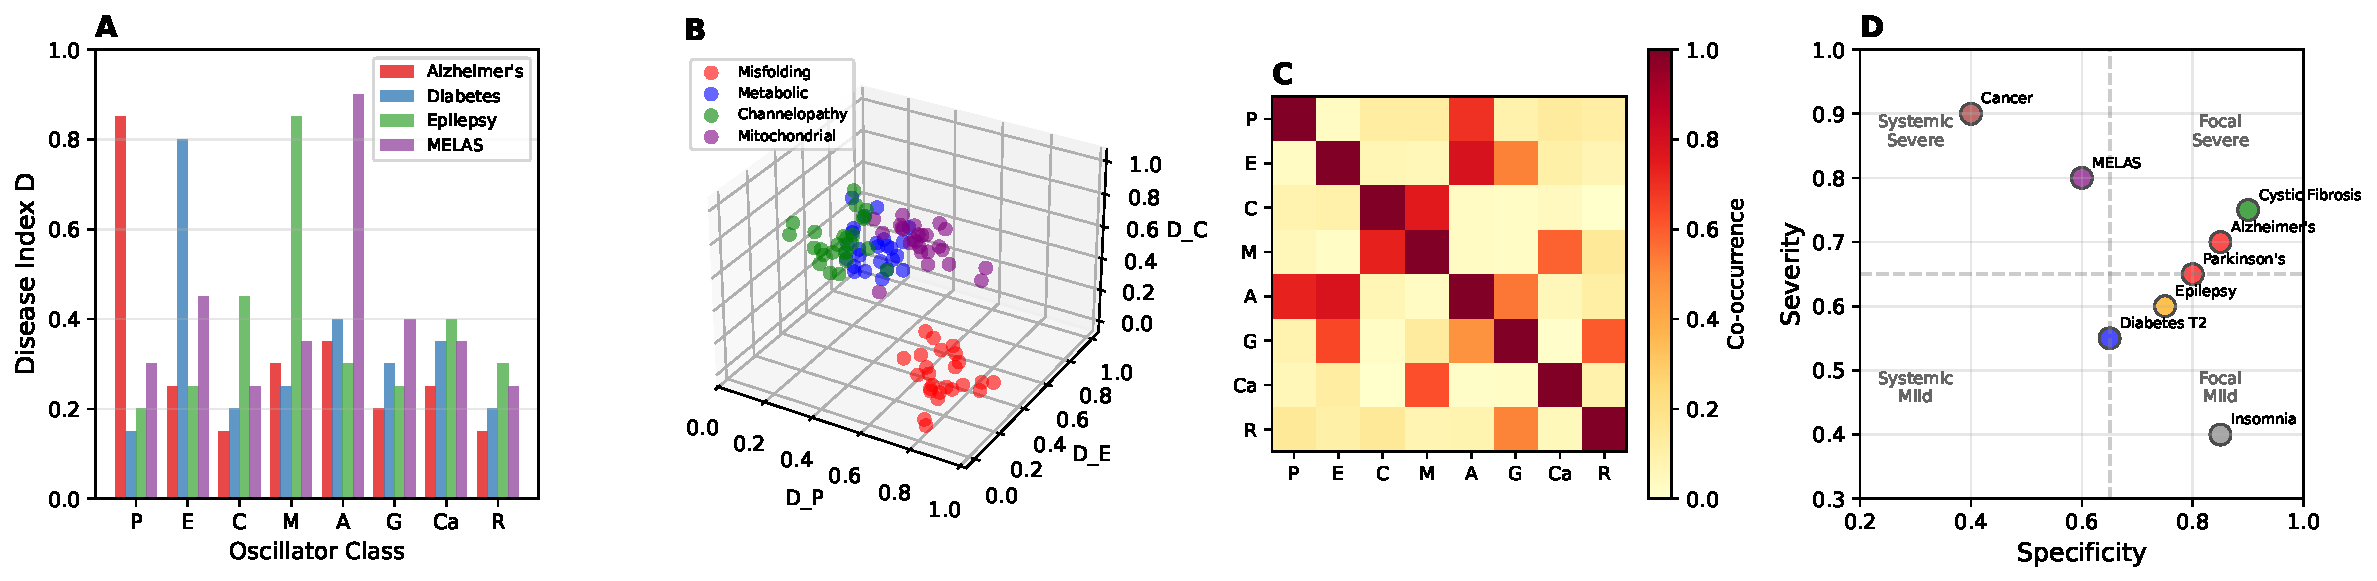
\includegraphics[width=0.9\textwidth]{figures/panel7_disease_taxonomy.pdf}
\caption{\textbf{Disease Taxonomy and Classification Structure.}
\textbf{Panel A (left):} Disease index profiles across eight oscillator classes (P: Protein/Misfolding, E: Enzyme/Metabolic, C: Channel, M: Membrane/Excitability, A: ATP/Mitochondrial, G: Genetic/Expression, Ca: Calcium/Signaling, R: Rhythm/Circadian) for exemplar diseases. Each disease exhibits a characteristic fingerprint with dominant dysfunction in its primary class.
\textbf{Panel B (center-left):} Three-dimensional disease taxonomy showing clustered populations in reduced disease space $(D_P, D_E, D_C)$. Distinct clusters emerge for misfolding (red), metabolic (blue), channelopathy (green), and mitochondrial (purple) disease categories, demonstrating geometric separability of disease types.
\textbf{Panel C (center-right):} Disease co-occurrence matrix showing correlation probabilities between oscillator class dysfunctions. Strong off-diagonal elements indicate biological coupling: metabolic-mitochondrial ($r = 0.7$), channel-membrane ($r = 0.65$), and misfolding-mitochondrial ($r = 0.6$) connections reflect known pathophysiological relationships.
\textbf{Panel D (right):} Taxonomic classification plot positioning diseases by specificity (single-class dominance) versus severity (total disease burden). Quadrants define focal/systemic and mild/severe categories, enabling systematic disease classification based on coherence measurements.}
\label{fig:disease_taxonomy}
\end{figure*}
